% Commande for better write
\makeatletter
\renewcommand*\l@author[2]{}
\renewcommand*\l@title[2]{}
\makeatletter
\newcommand{\reffig}[1]{n$^\circ$\ref{fig:#1}}
\newcommand{\refalg}[1]{n$^\circ$\ref{alg:#1}}
\newcommand{\intended}{\emph{intended}\xspace}
\newcommand{\enacted}{\emph{enacted}\xspace}
\newcommand{\intend}{\emph{intend}\xspace}
\newcommand{\enact}{\emph{enact}\xspace}
\newcommand{\radicalinteractionnism}{radical interactionnisme\xspace}
\newcommand{\actionInt}{\emph{action}\xspace}
\newcommand{\num}[1]{n$^\circ${#1}}
\newcommand{\triangleBlanc}{\protect
\includegraphics[width=0.02\textwidth]{triangle_blanc.pdf}}
\newcommand{\triangleBleu}{\protect
\includegraphics[width=0.02\textwidth]{triangle_bleu.pdf}}
\newcommand{\rondBlanc}{\protect
\includegraphics[width=0.02\textwidth]{rond_blanc.pdf}}
\newcommand{\rondBleu}{\protect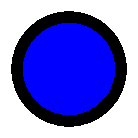
\includegraphics[width=0.02\textwidth]{rond_bleu.pdf}}
\newcommand{\carreBlanc}{\protect
\includegraphics[width=0.02\textwidth]{carre_blanc.pdf}}
\newcommand{\carreBleu}{\protect
\includegraphics[width=0.02\textwidth]{carre_bleu.pdf}}

